%%%%%%%%%%%%%%%%%%%%%%%%%%%%%%%%%%%%%%%%%%%%%%%%%%%%%%%%%%%%%%%%%%%%%%%%
%                                                                      %
%     File: Thesis_Implementation.tex                                  %
%     Tex Master: Thesis.tex                                           %
%                                                                      %
%     Author: Andre C. Marta                                           %
%     Last modified :  4 Mar 2024                                      %
%                                                                      %
%%%%%%%%%%%%%%%%%%%%%%%%%%%%%%%%%%%%%%%%%%%%%%%%%%%%%%%%%%%%%%%%%%%%%%%%

\chapter{Numerical Setup}
\label{chapter:numerical_setup}

In this chapter, we will describe the numerical setup of the \texttt{bamps} code. We will start by discussing the grid setup in section \ref{section:grid}, followed by the numerical method used to solve the partial differential equation systems in section \ref{section:Numerical_Method} and a brief description of how \texttt{bamps} handles patch boundaries in section \ref{section:Patch_Boundaries}. Finally, we will discuss the Adaptive Mesh Refinement (AMR) strategy employed by \texttt{bamps} in section \ref{section:amr}.

%%%%%%%%%%%%%%%%%%%%%%%%%%%%%%%%%%%%%%%%%%%%%%%%%%%%%%%%%%%%%%%%%%%%%%%%
\section{Grid Setup}
\label{section:grid}

The \texttt{bamps} code uses a multi-patch grid setup to cover the computational domain. Even though \texttt{bamps} is capable of supporting both a cubed-ball grid and a cubed-sphere grid, in this work we will only use the cubed-ball grid. The grid is composed of several patches which are shaped like deformed cubes that fit together to cover the domain. Each patch is mapped by two different coordinate systems: the local patch coordinates $(\bar{x},\bar{y},\bar{z})$ and the global Cartesian coordinates $(x,y,z)$.

The cubed-ball grid consists of a central cube surrounded by six deformed cube patches that form a spherical shell around the central cube forming a transition shell, which is itself surrounded by six more deformed cube patches that form the outer spherical shell. In the central cube, the local patch coordinates and the global Cartesian coordinates are identical, i.e., $(\bar{x},\bar{y},\bar{z}) = (x,y,z)$. However, in the other patches, a coordinate transformation must be applied to map the local patch coordinates to the global Cartesian coordinates. This transformation is performed in two steps: first, the local coordinates are transformed to temporary global coordinates $(\tilde{x},\tilde{y},\tilde{z})$, which are then transformed to the final global Cartesian coordinates $(x,y,z)$ by performing a rotation of the patch to their correct placement on the sphere. The transformation from local patch coordinates to temporary global coordinates is given by
%
\begin{align}
    x_t = \frac{\bar{x}}{\bar{s}} \; , \quad \quad y_t = \frac{\bar{x}}{\bar{s}} \bar{y} \; ,  \quad \quad z_t = \frac{\bar{x}}{\bar{s}} \bar{z} \; ,
\end{align}
%
where, for the outer patches,
%
\begin{align}
    \bar{s} = \sqrt{1 + \bar{y}^2 + \bar{z}^2} \; 
\end{align}
%
and for the inner patches,
%
\begin{align}
    \bar{s}(\lambda) = \sqrt{\frac{1 + 2\lambda}{1 + \lambda (\bar{y}^2 + \bar{z}^2)}} \; , \quad \quad \quad \lambda = \frac{\bar{x}^2 - \bar{x}_0^2}{\bar{x}_1^2 - \bar{x}_0^2} ,
\end{align}
%
where $\bar{x}_0$ and $\bar{x}_1$ are the boundaries of the patch in the local coordinates \cite{Pseudospectral_method_for_gravitational_wave_collapse}.

Each patch can be further divided into several subpatches, which are smaller cubes that allow for a more refined grid in specific regions of the domain. When dividing a patch into subpatches, the division is done such that subgrids of two neighboring patches match, and that neighboring patches and subpatches have the same grid-point positions on their respective boundaries. In figure \ref{fig:cubed_ball_grid}, we show an example of a cubed-ball grid divided into subpatches.

\begin{figure}[h]
    \centering
    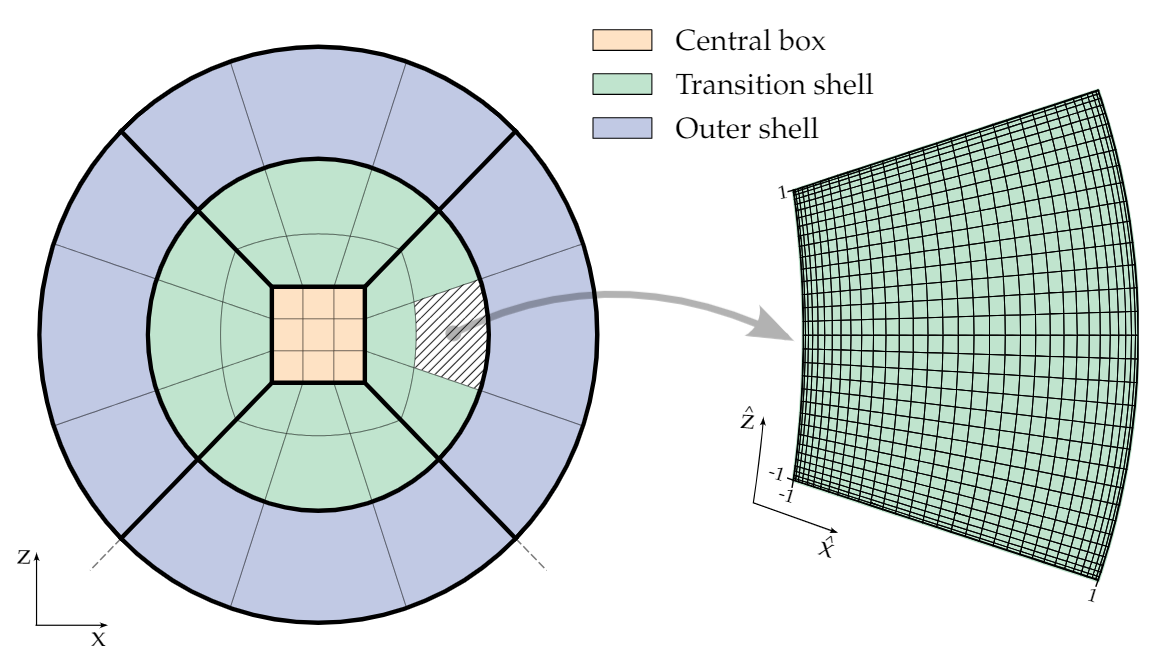
\includegraphics[width=0.8\textwidth]{Figures/Cubed_Ball.png}
    \caption{Two-dimensional sketch of the bamps cubed-ball grid layout. The grid is composed of several patches shaped like deformed cubes. These patches can be further divided into subpatches. Each subpatch is covered by Gauss-Lobatto grids. \cite{Pseudospectral_method_for_gravitational_wave_collapse}}
    \label{fig:cubed_ball_grid}
\end{figure}

%%%%%%%%%%%%%%%%%%%%%%%%%%%%%%%%%%%%%%%%%%%%%%%%%%%%%%%%%%%%%%%%%%%%%%%%
\section{Numerical Method}
\label{section:Numerical_Method}

\texttt{bamps} uses the method of lines to solve the system of partial differential equations, meaning that it treats time as a continuous variable and space as discrete. In order to integrate fields forward in time, a 4th order Runge-Kutta scheme is used. The spatial discretization is performed using Gauss-Lobatto collocation points, which is done by maping the local patch coordinates $(\bar{x},\bar{y},\bar{z})$ to the reference cube coordinates $(\tilde{x},\tilde{y},\tilde{z}) \in [-1,1]^3$ and then using the Gauss-Lobatto points in each direction. The Gauss-Lobatto points in the $\tilde{x}$ direction are given by
%
\begin{align}
    \tilde{x}_\alpha = - \cos\left(\frac{\pi \alpha}{N_x -1}\right) \; ,
\end{align}
%
with $\alpha = 0,1,\ldots,N_x -1$ and $N_x$ being the number of grid points in the $\tilde{x}$ direction. The collocation points in the other two directions are defined similarly. It is important to note that the number of angular grid points must be the same in all patches to ensure that the grid points on the boundaries of neighboring patches match \cite{Pseudospectral_method_for_gravitational_wave_collapse}. A grid generated using Gauss-Lobatto points can be seen in figure \ref{fig:cubed_ball_grid}.

On each of the colocation points, all the evolution fields $u$ are expanded in each dimension in terms of Chebyshev polynomials $T_n(\tilde{x})$ as
%
\begin{align}
    u_{\alpha \beta \delta} = u(\tilde{x}_\alpha, \tilde{y}_\beta, \tilde{z}_\delta) = \sum_{l=0}^{N_z -1} c^x_n(\tilde{y}_\beta, \tilde{z}_\delta) \, T_n(\tilde{x}_\alpha) \; ,
\end{align}
%
and similarly for the $\tilde{y}$ and $\tilde{z}$ directions. \texttt{bamps} uses the pseudospectral approach, meaning that instead of storing the coefficients $c^x_n(\tilde{y}_\beta, \tilde{z}_\delta)$, it stores the values of the fields at the collocation points. The spatial derivatives of the fields are computed using matrix multiplication. For example, the derivative in the $\tilde{x}$ direction is computed as
%
\begin{align}
    (\partial_{\tilde{x}} u)_{\alpha \beta \delta} = \sum_{n=0}^{N_x -1} D_{\alpha n} u_{n \beta \delta} \; ,
\end{align}
%
where $D_{\alpha n}$ is the Gauss-Lobatto differentiation matrix
%
\begin{align}
    D_{\alpha\beta}=
    \begin{cases}
    -\frac{2(N_x-1)^2+1}{6} & \alpha=\beta=0 \\
    \frac{q_\alpha}{q_\beta}\frac{(-1)^{\alpha+\beta}}{\tilde{x}_\alpha-\tilde{x}_\beta} & \alpha\neq\beta \\
    \frac{-\tilde{x}_\beta}{2(1-\tilde{x}_\beta^2)} & \alpha=\beta=1,\cdots,N_x-2 \\
    \frac{2(N_x-1)^2+1}{6} & \alpha=\beta=N_x-1
    \end{cases} \, ,
\end{align}
%
where $q_\alpha = 2$ on the boundaries and $q_\alpha = 1$ otherwise \cite{Pseudospectral_method_for_gravitational_wave_collapse}.

In order to ensure numerical stability, \texttt{bamps} uses a filtering method to remove high-frequency modes. The filtering is applied after each full time step and consists of multiplying the fields with a filter matrix in each direction
%
\begin{align}
    (\mathcal{F}u)_{\alpha \beta \delta} = \sum_{n=0}^{N_x -1} \mathcal{F}_{n \alpha} u_{n \beta \delta} \; ,
\end{align}
%
where the filter matrix $\mathcal{F}_{n \alpha}$ is given by
%
\begin{align}
    \mathcal{F}_{\alpha \beta} = \sum_n S_{\alpha n} e^{-36 (n/(N_x - 1))^{64}} A_{n \beta} \; ,
\end{align}
%
where $S_{\alpha \beta}$ is the Chebyshev synthesis matrix and $A_{n \beta}$ is Chebyshev analysis matrix \cite{Pseudospectral_method_for_gravitational_wave_collapse}.

%%%%%%%%%%%%%%%%%%%%%%%%%%%%%%%%%%%%%%%%%%%%%%%%%%%%%%%%%%%%%%%%%%%%%%%%
\section{Patching Boundary Conditions}
\label{section:Patch_Boundaries}

Since $\texttt{bamps}$ separates our domain into different patches, we need to impose boundary conditions between adjacent patches so that they can communicate data to each other. An effective way to impose these boundary conditions is to add appropriate penalty terms to the equations on these boundaries. This method, which we call \textit{Penalty Method}, imposes the needed boundary conditions while keeping the evolution equations at the boundary almost unchanged \cite{Pseudospectral_method_for_gravitational_wave_collapse,Spectral_methods_for_the_wave_equation_in_second-order_form}.

It consists of adding to the equation of motion of the incoming characteristic variable a term of the form $(u_-^{BC}  - u_-)$, where $u_-$ is the incoming \textit{characteristic variable}. Thus, if the boundary condition $u_-^{BC} = u_-$ is satisfied, the penalty terms vanish. We can then determine the appropriate penalty terms to add to the equation when written in their fundamental form by rewriting our evolution equations on the boundaries as functions of the characteristic variables, incorporating the penalty terms, and then transforming our system back \cite{Pseudospectral_method_for_gravitational_wave_collapse,Spectral_methods_for_the_wave_equation_in_second-order_form}. That way, the evolution equations \eqref{eq:wave_equation_3+1} on the boundary will get modified to
%
\begin{align}
    \left\{\begin{array}{@{}l@{}} 
        (\partial_t\tilde{\psi})^{BC} = \partial_t\tilde{\psi} \\
        (\partial_t\tilde{\Pi})^{BC} = \partial_t\tilde{\Pi} + \frac{1}{2} p \, \left( v_+(u_+^{BC}  - u_+) + v_- (u_-^{BC}  - u_-) \right) \\
        (\partial_t\tilde{\phi}_i)^{BC} = \partial_t\tilde{\phi}_i + \frac{1}{2} p \, n_i \, \left( v_+(u_+^{BC}  - u_+) - v_- (u_-^{BC}  - u_-) \right)  + p \, v_2 \left((u_2^{BC})_i  - (u_2)_i \right) \\
    \end{array}\right. ,
    \label{eq:penalty_terms}
\end{align}
%
where $p$ is the penalty coefficient, which can determined from a semi-discrete energy analysis, and $n^i$ is the unit outgoing normal vector to the boundary. Even though in equation \eqref{eq:penalty_terms} the terms regarding every characteristic variable are included, it is important to note that only incoming characteristic variables are taken into account in this method, thus if any of the characteristic speeds are greater than $0$, the penalty term associated will be null. 

If we allow for constraint violations in our system (as we did in equation \eqref{eq:wave_equation_constraint_violation}), the characteristic variables and their respective speeds will change, and we will need to modify the penalty terms accordingly, obtaining
%
\begin{align}
    \left\{\begin{array}{@{}l@{}} 
        (\partial_t\tilde{\psi})^{BC} = \partial_t\tilde{\psi} - p \, v_0 (u_0^{BC}  - u_0)\\
        (\partial_t\tilde{\Pi})^{BC} = \partial_t\tilde{\Pi} + \frac{1}{2} p \, \left( v_+(u_+^{BC}  - u_+) + v_- (u_-^{BC}  - u_-) \right) - 2 \, \gamma_2 \, p \, v_0 (u_0^{BC}  - u_0)\\
        (\partial_t\tilde{\phi}_i)^{BC} = \partial_t\tilde{\phi}_i + \frac{1}{2} p \, n_i \, \left( v_+(u_+^{BC}  - u_+) - v_- (u_-^{BC}  - u_-) \right)  + p \, v_2 \left((u_2^{BC})_i  - (u_2)_i \right) \\
    \end{array}\right. .
\end{align}

%%%%%%%%%%%%%%%%%%%%%%%%%%%%%%%%%%%%%%%%%%%%%%%%%%%%%%%%%%%%%%%%%%%%%%%%
\section{Adaptive Mesh Refinement}
\label{section:amr}

